\chapter{Full text Search}

The aim of this chapter is to explain basic concepts applied in full
text search, one of the methods dealing with the problem of searching information.

\section{Information retrieval}

Full text search together with database systems can be considered  as a part of a subdiscipline of computer science known
as information retrieval (IR) \cite{Witten:1999:MGC:323905}.
There is a number of available definitions of information retrieval.
According to \cite{IRDataAlgorithms}, information
retrieval (IR) is loosely defined as

	\begin{quote}
		\textsl{``the subfield of computer science
	that deals with the automated storage and retrieval of documents''}
	\end{quote}

This definition as well as the definitions from other sources (e.g. from \cite{Witten:1999:MGC:323905}) sum up the purpose of IR in a very general way.
While the definition above puts no restrictions to the nature of stored documents in the IR system and therefore comprises both full text search and database systems, there exist stricter IR definitions that do not apply to structured data found typically in relational databases. 
Such definition of IR can be found in \cite{Manning:2008:IIR:1394399}:

	\begin{quote}
		\textsl{``Information retrieval (IR) is finding material (usually documents) of an unstructured nature (usually  text) that satisfies an information need from within large collections (usually stored on computers).''}
	\end{quote}

All IR systems - and full text search engines are no exception - are based on the same architecture which is adapted to requirements the specific systems have. In addition, these systems share common IR terminolgy, whose most important terms are explained in this chapter.

\section{Principles of Full Text Search}

% Ostry text

The field of full text search covers a wide range of topics, including efficient algorithms and data structures in order to enable fast and reliable full text search over large amount (in practice gigabytes) of data. 
It is not the aim of this thesis to provide a deeper, more complex insight into this problematics as the final implementation of the full text search feature will be based on an existing full text search engine. 
However, there are several terms and concepts that must be at least briefly explained so that the reader can fully understand the latter text.


\subsection{Full Text Search Engine Architecture}

As can be seen in schema in Figure ~\ref{fig:fulltext_schema}, full text search engines comprise several steps in order to provide a user with search results to a given \textsl{query}. 
\textsl{Query} is in this case a piece of text to be searched, optionally enriched by special operators which serve for refining the query. It is a \textsl{user} of the IR system who comes up with the query, expecting that the system will fulfill his \textsl{information need} by returning relevant search results.

Search engines need source data to actually perform searching. The basic informational unit which is processed by the search engine and returned to the user in case of match with the query is called \textsl{document}. In this context, a document or a collection of documents inserted to the system are representations of real documents, so a series of data transformations must be made first. These steps are for reasons of clarity not depicted in the schema.
  
\begin{figure}[h]
	\centering
		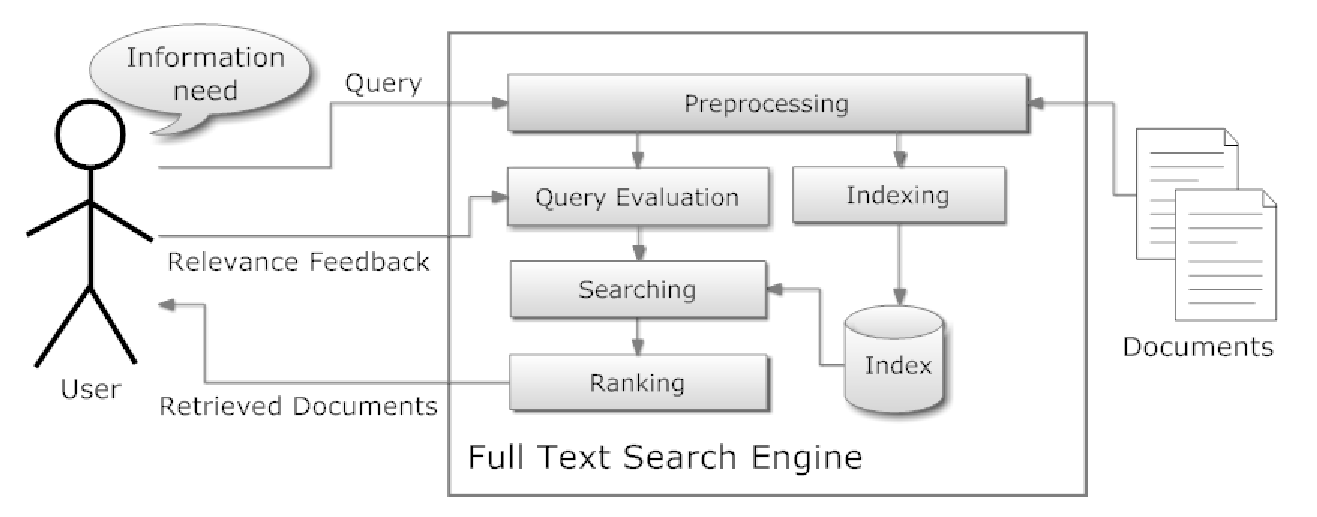
\includegraphics[scale=0.63]{figures/fulltext_schema.eps}
	\caption{IR Architecture Schema. Adapted from \cite{IR:ImplemEvalSearchEng}.}
	\label{fig:fulltext_schema}
\end{figure}

TODO vysvetlit schema, pojmy nize - in progress...

\subsubsection{Preprocessing phase}

Both input query and documents usually undergo several preprocessing steps. These steps, sometimes reffered to as \textsl{filters},   
treat the input text as a stream. 

Tokenization = token stream -> tokens; token normalization -> lowercasing letters, removal of accents, diacritics and so on

separate the text into basic textual units called \textsl{tokens}, in some sources also reffered to as \textsl{words}. These tokens are then operated on. The operations can involve. The result of these operations is a set of terms which are kept in a lexicon of the IR system. 

\subsubsection{Indexing phase}

\subsubsection*{Index}

Index is defined by Frakes \cite{IRDataAlgorithms} the following way: 
	\begin{quote}
	\textsl{``A collection of terms with pointers to places where information about them can be found.''} 	
	\end{quote}
Based on information found in \cite{ManningRaghavanSchuetze08, IRDataAlgorithms, Witten:1999:MGC:323905}, there are three main indexing methods – inverted file, signature file and bitmaps. Based on the comparisons made \cite{Witten:1999:MGC:323905} and in \cite{Zobel:1996:GPC:234889.234891}, using inverted files should be the prefered way due to their faster speed and lower index size required. The remaining two alternatives are recommended to be used only in certain circumstances which are very rare in practice. 

\subsubsection*{Inverted File}

This data structure can be thought of as the well-known index at the end of a book. If we sticked to the IR terminology and characterize it more precisely, we might come up with a more precise characteristics, such as the one found in \cite{Witten:1999:MGC:323905}:

\begin{quote}
		\textsl{``An inverted file contains, for each term in the lexicon, an inverted list that stores a list of pointers to all occurrences of that term in the main text, where each pointer is, in effect, the number of a document in which that term appears.''}
	\end{quote}
	
	To visualize the basic idea of the invered file, Figure  represents a situation of an indexed sentence.
	Obrazek!!!
	
\subsubsection{Query evaluation}

\subsubsection{Searching phase}


\subsubsection*{Boolean query}

\subsubsection*{Ranked query}


\subsubsection{Ranking phase}	


\subsubsection*{Query, Term, Document Operations}

\subsubsection*{Relevance Evaluation}

\subsubsection*{Filters}


% Poznamky

%An IR system matches user queries - formal statements of information
%needs - to documents stored in a database. {[}IRDSA,Frakes{]}
%
%An IR system must support certain basic operations. There must be
%a way to enter documents to a database, change the documents and delete
%them.The must be also some way to search for documents, and present
%them to a user.
%
%and to overcome the informational overload
%
%Though it is possible to keep the index structure in main memory,
%in practice IR databases are usually stored on disk because of their
%size.
%
%Inverted file - a kind of indexed file, the most common solution in
%commercial systems {[}IRDSA,Frakes{]}
%
%The basic item stored in the index 
%
%Todo Lucene in Action and other sources
%
%identify index terms
%
%how to decide if a document matches a query
%
%precision = number of relevant documents retreived divided by the
%total number of documents retreived
%
%recall = number of relevant documents retreived divided by the total
%number of relevant documents
%
%ideally, both parameters should equal to one. This would mean that
%the system returns all relevant documents without introducing any
%irrelevant documents in the results set - impossible to acheive in
%practice.
%
%Improving recall -> precision decreases, likewise improving precision
%at the expense of recall
%
%Furthermore - tradeoff between retreival effectiveness and computing
%cost (key word matching < statistical ranking <\ natural-language
%processing)
%
%Statistical model
%
%Here a document is conceptually represented by a vector of keywords
%extracted from the document, with associated weights representing
%the importance of the keywords in the document and within the whole
%document collection.
%
%Query is modelled as a list of keywords with associated weights representing
%the importance of the keywords in the query.
%

\section{Full text vs. DB search}

Relational database systems and their properties ACID - widely used
for structured data, they are a perfect fit for storing structured
data. As long as these conditions are met relational databases are
a recommended solution for our domain.

traditional search engines - e.g. MySQL databaze. Je zde konstrukce
LIKE (LIKE '\%life\%').

If more terms are searched the underlying query grows in complexity.
Multiple JOIN operations must be used to fetch all data from corresponding
tables, also the query must be written the way to ensure finding the
records with terms not necessarily next to each other as well. As
the query gets more complex, it takes more time to get query results.
Furthermore, the query execution slows down due to the fact that the
query needs to match each term individually.

The query result does not contain any information on the relevancy
of searched terms and found results. Relational database systems simply
output the records matching the criteria.

On the contrary, IR systems provide us with additional relevancy information
of searched terms. Document relevancy is one of the key features of
full text search engines because it is desired to display the results
sorted by their relevance (mostly those most relevant ones are displayed
first).

It is worth mentioning that some DBMS posess native full-text support.
MySQL - keyword FULLTEXT INDEX, for searching on a field, on which full text search will be performed. 
These fulltext indexes are supported only by 
MyISAM engine. They are generally faster than LIKE, however, their usage is limited - vendor lock-in,
moreover, this solution is not unified (implementace,syntaxe se mouhou
can differ, decision to switch to another database could mean interactions to the current system to preserve functionality and scalability. It is bound solely to DBMS - they also lack bigger scaling possibilities and have problems in this area. And it is still slower than external search engines.

{[}IRDSandA,Frakes, p.14{]}:

difference - amount of usable structure in their data objects. Document
generally have less usable structure than the table used by relational
DBMS.

IR - retrieval is probabilistic. No certainity that a retreived document
will meet the informaiton need of the user. (typically, some relevant
documents will be missed, whereas some nonrelevant documents wil be
retreived) vs. DB queries consist of attribute-value pairs that either
match or do not match records in the database.

same - their databases are often very large (can be gigabytes)

same - database volatility - means constant changes as documents are
added, changes or deleted.


\section{Benefits of full text search}

When searching over unstructured data and large data sets, full text
search should be favored to querying relational databases.
\begin{itemize}
\item faster than traditional database search - benefits from word index,
ktery se prochazi pri hledani (jsou pouzity to look up records),
vs. DB - provadi se full table scan
\item found records can be sorted by their relevance. This is called ranking.
\item good performance also over a DB with millions of records
\item ability to skip common words with no additional information. This
depends on the domain languages (in case of English these words include
e.g. the, an, for), search precision can decrease in some cases. 
\end{itemize}
Fulltext pouzijeme, pokud:
\begin{itemize}
\item if there is a lot of unstructured data that are to be looked up
\item it is necessary to get optimized search results.
\item demand for flexible querying
\end{itemize}

\section{Search Engines}

It is a software that is responsible for two steps:
\begin{itemize}
\item building an index on text
\item answering queries by using the created index
\end{itemize}
Compared to databases, it beats them by scalability, relevance ranking,
integration of different data sources (email, web pages, files, database,
...)


\section{Indexing}

Despite various specifics of available search engines, the indexing proces generally consists of several phases.
\cite{Fox:1991:FFA:903195}


\section{Searching Features}

Todo
